\documentclass[11pt]{article}

\usepackage{amsmath}
\usepackage{textcomp}
\usepackage[top=0.8in, bottom=0.8in, left=0.8in, right=0.8in]{geometry}

% add other packages here
\usepackage{amssymb}
\usepackage{mathtools}
\usepackage{graphicx}
\usepackage{subcaption}
\usepackage[export]{adjustbox}
\newcommand{\R}{\mathbb{R}}
\newcommand{\N}{\mathbb{N}}

% put your group number and names in the author field
\title{\bf Exercise 2: A Reactive Agent for the Pickup and Delivery Problem}
\author{Group \textnumero$75$: Thomas KIMBLE, Jules AFRESNE}

% the report should not be longer than 3 pages

\begin{document}
\maketitle

\section{Problem Representation}

\subsection{Representation Description}
% describe how you design the state representation, the possible actions, the reward table and the probability transition table

\indent \indent Our state representation design is done by initialising a $N * N$ matrix, $N$ being the number of cities in a topology as shown below. We initialise the diagonal of this matrix ($S_{ij}$ with $i=j$) as having no package and being in city $i=j$. The rest ($S_{ij}$ with $i \neq j$) are initialised as being in city $i$ with a package destined to city $j$.
\[
State = \begin{bmatrix} 
    S_{11} & \dots & S_{1N}\\
    \vdots & \ddots & \\
    S_{N1} &        & S_{NN} 
    \end{bmatrix}
\]
\\
\\
\indent Our possible actions are designed by initialising an array of size $(N+1)$ (considered a $1*(N+1)$ matrix), $N$ still being the number of cities in a topology. We fill the first $N$ values of the array with the list of cities in the topology, here the agent does not want to take a delivery and wants to move in city $i$ thanks action $a_i$. The final value of the array, $a_{N+1}$, is the action to take a delivery.
\[    
action = \begin{bmatrix}
    \smash[b]{\underbrace{\begin{matrix}a_1 & a_2 & \dots  & a_N \end{matrix}}_{N\text{ cities}}}
    \smash[b]{\underbrace{\begin{matrix}a_{N+1}\end{matrix}}_{\text{Take Delivery}}}
    \end{bmatrix}
\]
\\
\\
\indent Our reward table is designed with three cases. First of all, if the agent does not have a package and refuses to take a delivery, his reward is the negative of the distance to a neighbouring city (equation 1). Secondly, if the agent is looking for a package but no package is available in the city, his reward is also the negative of the distance to a neighbouring city (equation 1). Finally, if the agent does have a package and completes the delivery, his reward is the reward $R_i_j$ for a task that is transported from city $i$ to city $j$, defined by the $TaskDistribution$, minus the distance between the destination city and the previous city (equation 2). We add an "infinite" negative reward for any other state/action combinations to avoid impossible situations. Note that for equations 1 and 2 we have coefficients $C\in \R$ to be determined during experiments.
\[
    Reward = - C\cdot Distance \; \; \; \; \text{(1)} \; \; \; \; \; \; \; \; \; \; \; \; \; \; \; \; \; \; \; Reward = R_t_a_s_k - C\cdot Distance \; \; \; \;  \text{(2)}
\]
\\
\indent Our probability transition table is designed as following. We notice that while in a state with no package in the city ($S_{ij}$ with $i=j$), it is impossible to take the "Take Delivery" action ($a_{N+1}$). Therefore we give this combination a probability $p=0$. It is also impossible to move to the same city, therefore action $a_i$ while in state $S_{ij}$ ($i\neq j$) is also impossible and therefore takes a probability $p=0$. The other transition probabilities are obtained from the $TaskDistribution$ class.

\begin{figure}[h]
    \centering
    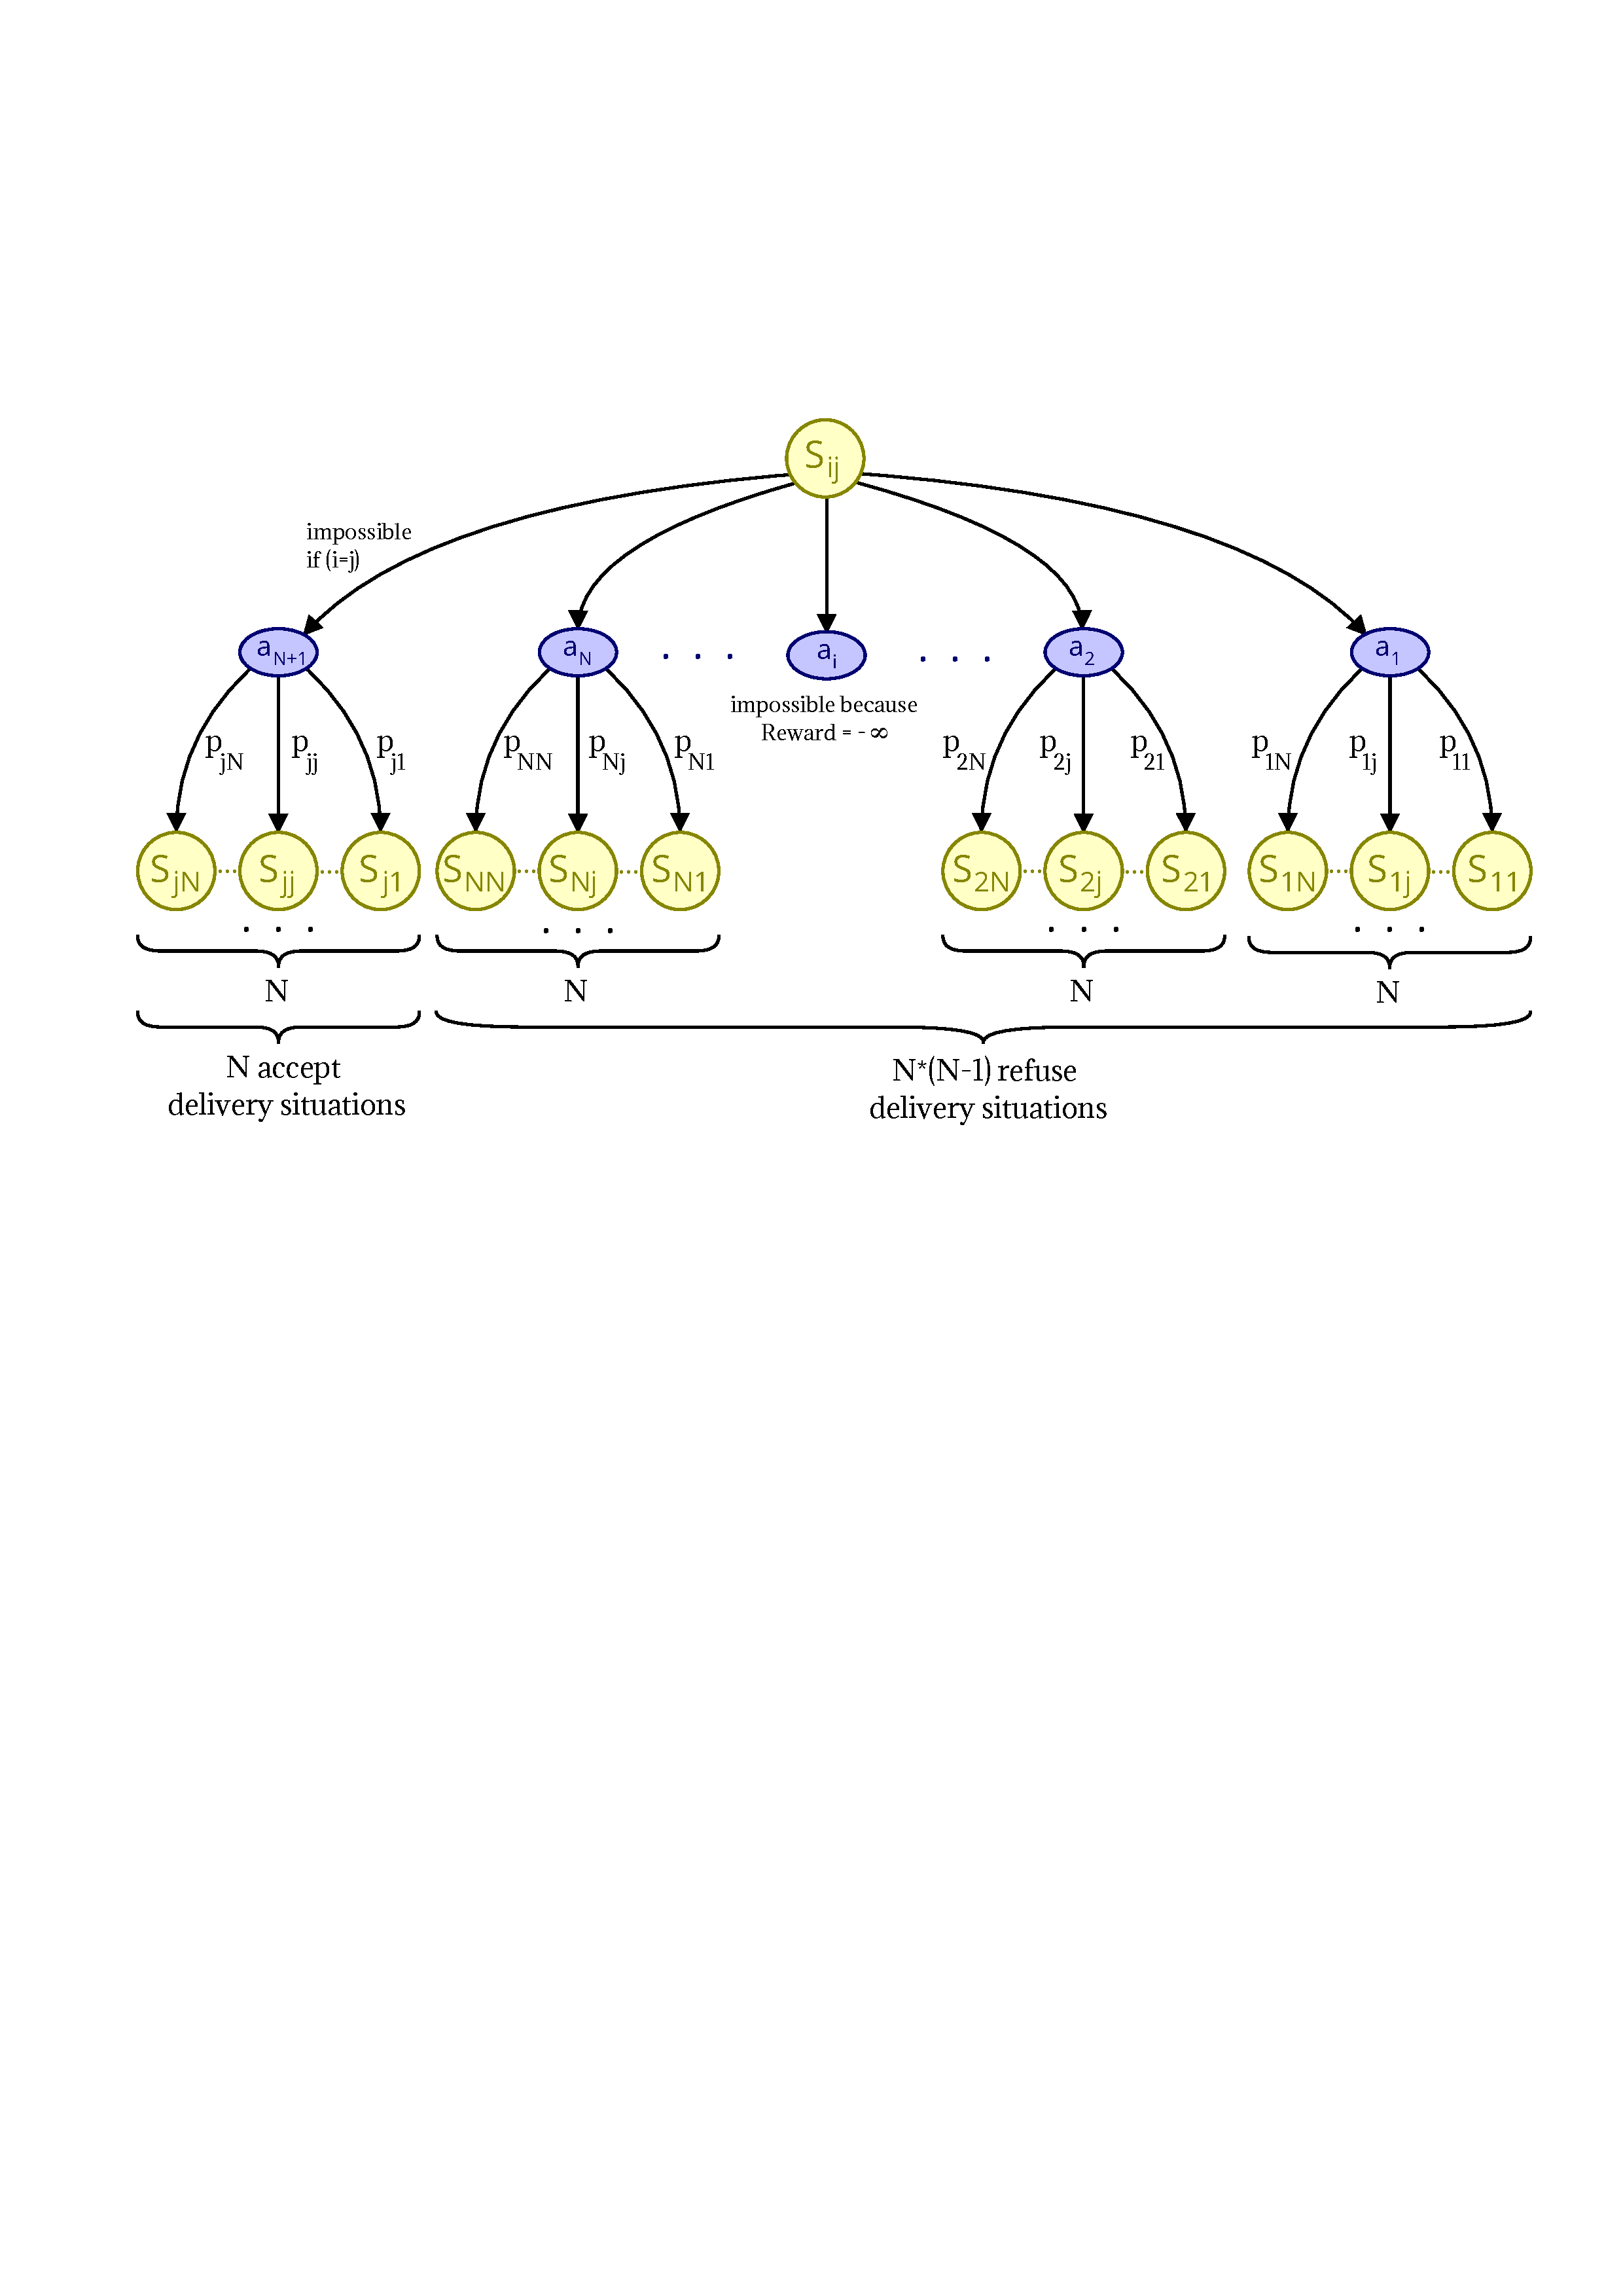
\includegraphics[width=0.7\textwidth, frame]{Fig1.pdf}
    \caption{State-Action diagram with Probabilities ($i, j \in \N$ and $<N$, the number of cities in a topology)}
    \label{fig:1}
\end{figure}

\subsection{Implementation Details}
% describe the implementation details of the representations above and the implementation details of the reinforcement learning algorithm you implemented

\indent \indent We created two additional classes for the implementation of our reactive agents: $StateObj$ and $ActionObj$ that represent the features of states and actions available. To implement the policy we use matrices (2D-array) that first we have initialised and then we have computed them following the algorithm given.

\section{Results}
% in this section, you describe several results from the experiments with your reactive agent

\subsection{Experiment 1: Discount factor}
% the purpose of this experiment is to understand how the discount factor influences the result

\subsubsection{Setting}
% you describe how you perform the experiment (you also need to specify the configuration used for the experiment)

\indent \indent To see the influence of the discount factor we created a simulation with multiple agents with different discount factors from $\gamma=0.1$ to $\gamma=0.95$, with increments of 0.05 in between. Let's consider Reward per km to determine performance. Over multiple experiments placing the agents in different starting positions with different discount factors and a time of 20'000 clicks at $SimSpeed = 100$ we observe the following. (Note that all of this is done without changing the coefficient defined in part 1.1).

\subsubsection{Observations}
% you describe the experimental results and the conclusions you inferred from these results

\indent \indent The best performing agent here has a discount factor of $\gamma = 0.9$ which will now consider our optimal discount factor. The Reward per km reaches a stable 66 as opposed to 63 for the lower performing agents.

\subsection{Experiment 2: Coefficient determination}

\subsubsection{Setting}

\indent \indent In our representation the reward follows equations 1 and 2 as described in part 1.1. We modify the coefficient $C$ to different values, run the experiment for 5'000 clicks at $SimSpeed = 100$. We use $C_1 = 1$, $C_2 < 1$, $C_3 > 1$ and $C_4 >> 1$ and observe the following.

\subsubsection{Observations}

\indent \indent We can clearly see in Figure 2 that the reward per km increases with a high coefficient, and stays the same for values around $1$. However the average profit decreases with a higher coefficient. This is because a high coefficient punishes long distances, therefore the agent values shorter journeys with lower rewards over longer journeys with higher rewards (average profit is around 3900 for low $C$ and around 3400 for high $C$). If we are looking for a long term investment, a high Reward per km is more interesting. We hereby choose a coefficient $C=70$ to get a Reward per km of around 90.

\begin{figure}[h]
    \centering
    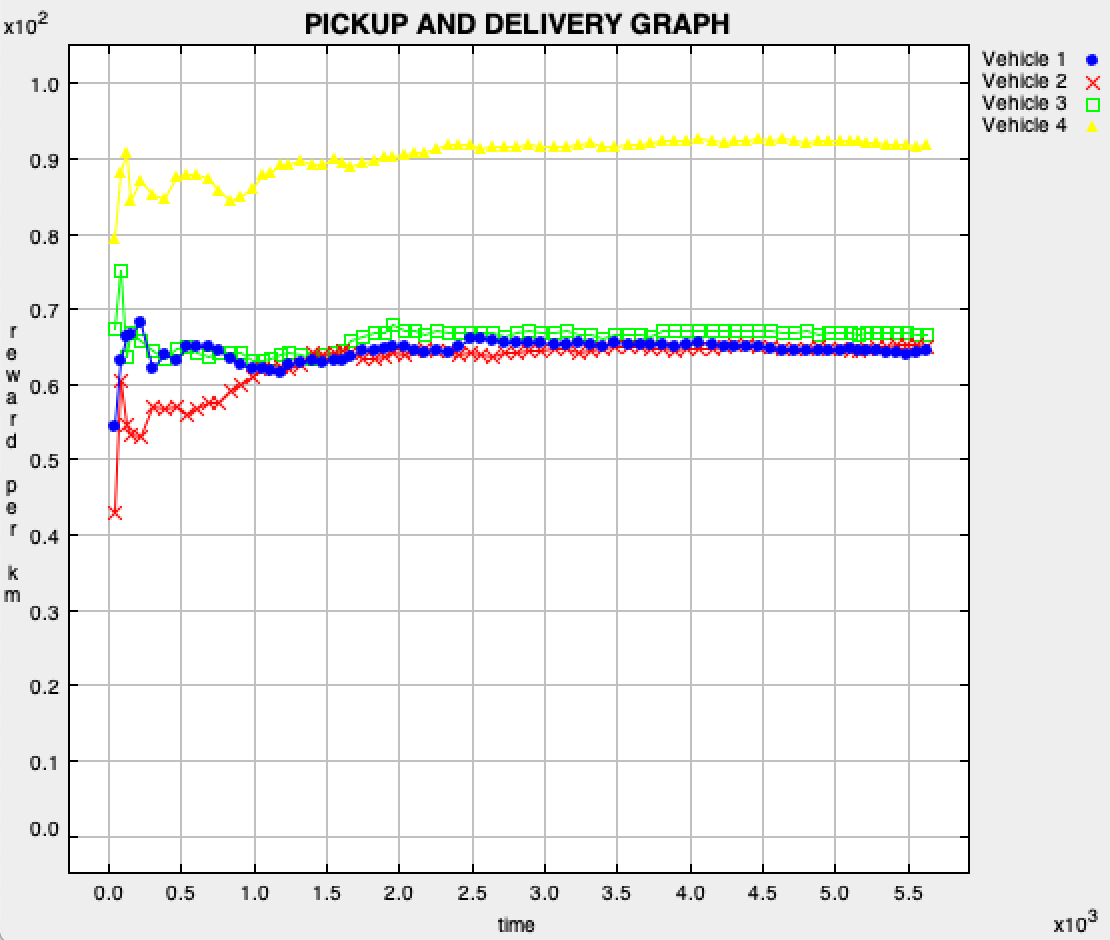
\includegraphics[width=0.35\textwidth, frame]{Fig2.png}
    \caption{Reward per km as a function of time with vehicle 1 (blue): $C_1 = 1$, vehicle 2 (red): $C_2 < 1$, vehicle 3 (green): $C_3 > 1$ and vehicle 4 (yellow): $C_4 >> 1$}
    \label{fig:1}
\end{figure}

\subsection{Experiment 3: Comparisons with dummy agents}
% you compare the results of your agent with two dummy agents: the random agent that was already given in the starter files and another dummy agent that you define and create. You should report the results from the simulations using the topologies given in the starter files and optionally, additional topologies that you create.

\subsubsection{Setting}
% you describe how you perform the experiment and you describe the dummy agent you created (you also need to specify the configuration used for the experiment)

\indent \indent We use the random agent given, our reactive agent with $\gamma=0.9$ and $C=70$, and our dummy agent is a reactive agent with $\gamma=0.5$ and $C=1$. We observe the following for two topologies: France (Figure 3a) and England (Figure 3b).

\subsubsection{Observations}
% elaborate on the observed results
\begin{figure}[ht]
\begin{centering}
  \begin{subfigure}[t]{0.36\textwidth}
    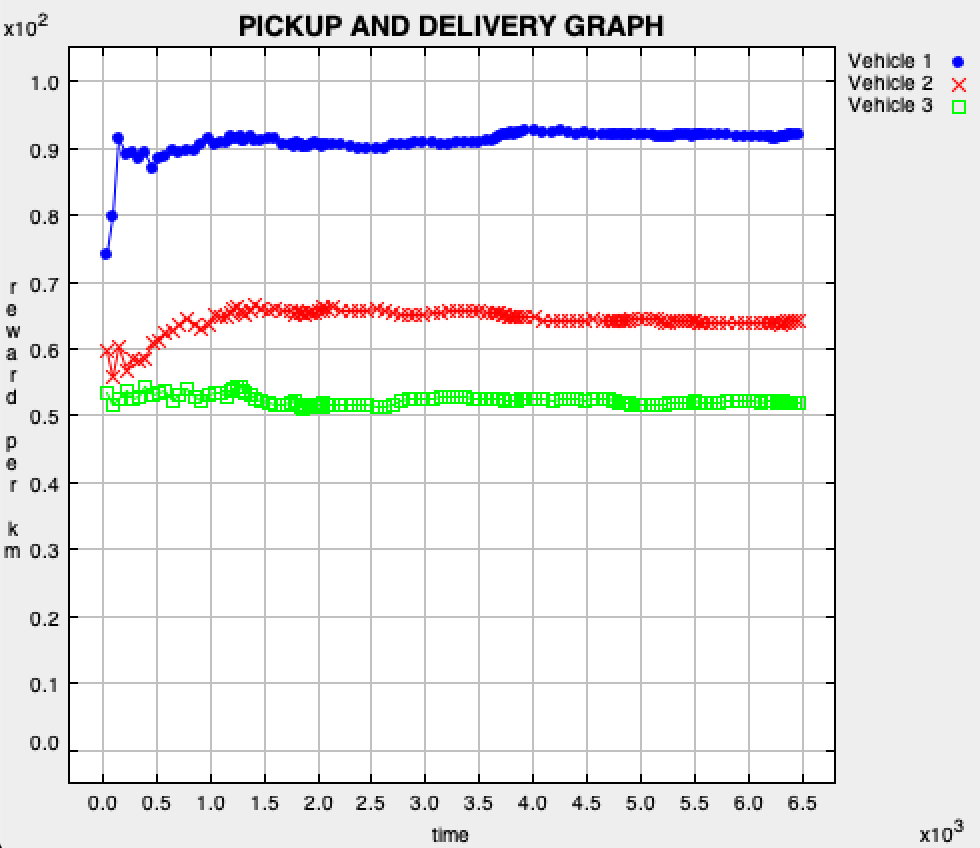
\includegraphics[width=\textwidth, frame]{Fig3a.png}
    \caption{Topology: France}
    \label{fig:3a}
  \end{subfigure}
  %
  \begin{subfigure}[t]{0.35\textwidth}
    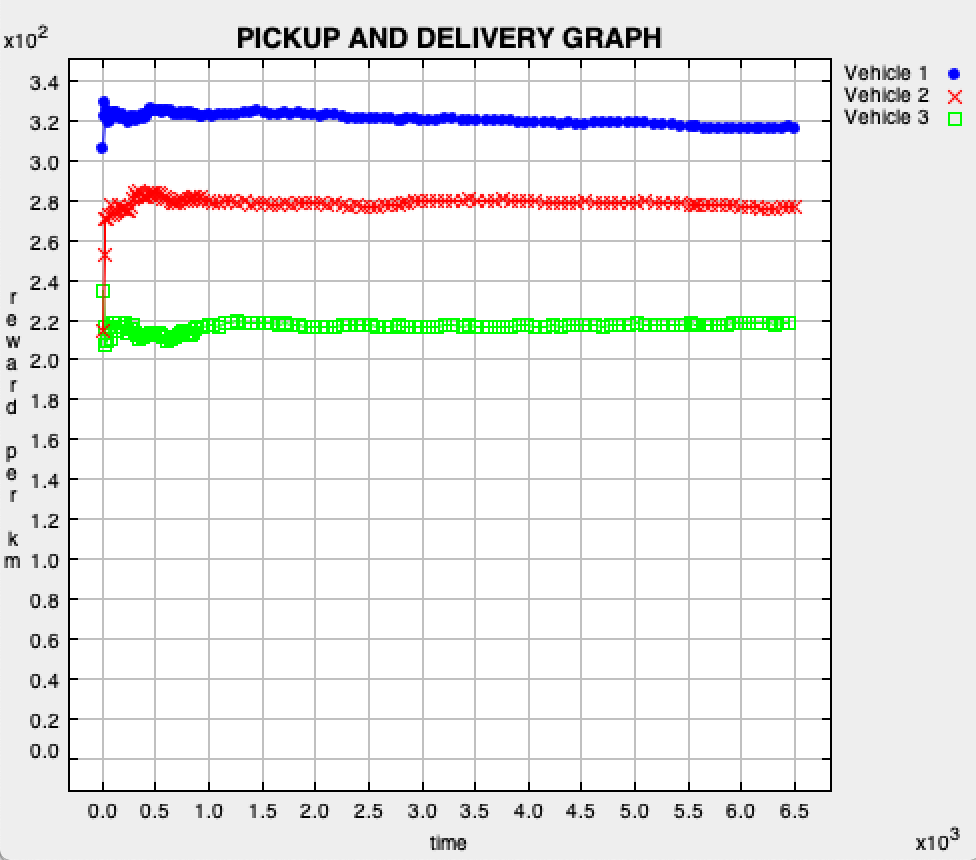
\includegraphics[width=\textwidth, frame]{Fig3b.png}
    \caption{Topology: England}
    \label{fig:3b}
  \end{subfigure}
  \label{fig:5}\caption{Reward per km as a function of time with Reactive Agent (blue), Dummy Agent (Red), and Random Agent (green)}
  \end{centering}
\end{figure}

\noindent In all cases, our agent outperforms the dummy and the random.

\end{document}